\chapter{Il Modello ad Attori e Akka}

\section{Fondamenti della Computazione Concorrente e Distribuita}

\subsection{La Crisi della Concorrenza e il Paradigma a Memoria Condivisa}
Le architetture computazionali moderne sono intrinsecamente parallele. Il raggiungimento dei limiti fisici di dissipazione termica e di densità di potenza (il cosiddetto \textit{"power wall"}) ha imposto l'arresto della scalabilità della frequenza di clock dei singoli processori. L'industria dell'hardware ha risposto deviando lo sviluppo verso architetture multi-core, many-core e sistemi distribuiti su larga scala. Di conseguenza, l'ottenimento di un elevato throughput e di una bassa latenza nell'elaborazione del software richiede l'adozione di modelli di esecuzione concorrente.

Storicamente, l'astrazione dominante per la programmazione concorrente su sistemi a memoria condivisa (\textit{shared-memory}) è stata il multi-threading affiancato da primitive esplicite di sincronizzazione (quali lock di mutua esclusione, semafori, monitor e operazioni atomiche in memoria). In tale modello, più thread concorrenti condividono un unico spazio di indirizzamento virtuale, accedendo e mutando direttamente le medesime locazioni di memoria. Tuttavia, questo approccio manifesta gravi patologie sia teoriche sia ingegneristiche:
\begin{enumerate}
    \item \textbf{Interleaving Non Deterministico e Race Condition}: L'ordine temporale degli accessi concorrenti alla memoria è governato dallo scheduler dei thread del sistema operativo e dai modelli di memoria hardware (store buffer, esecuzione fuori ordine e ottimizzazioni del compilatore). Se due o più thread accedono contemporaneamente alla medesima locazione di memoria senza opportuna sincronizzazione e almeno un accesso è in scrittura, si verifica una \textbf{race condition} (corsa critica). Rilevare, riprodurre e risolvere tali anomalie è notoriamente complesso a causa della natura non riproducibile dei diversi interleaving di esecuzione.
    \item \textbf{Deadlock, Livelock e Contesa dei Lock}: Il coordinamento degli accessi a risorse condivise multiple impone gerarchie globali e rigorose di acquisizione dei lock per scongiurare condizioni di attesa circolare (le note condizioni di Coffman per il deadlock). All'aumentare della complessità del sistema, mantenere coerenti tali gerarchie diviene intrattabile. L'adozione di lock a grana fine (\textit{fine-grained locking}) introduce elevata latenza di sincronizzazione, contesa di cache (cache bouncing) e alto rischio di deadlock, mentre lock a grana grossa (\textit{coarse-grained locking}) serializzano l'esecuzione, distruggendo i vantaggi prestazionali del parallelismo.
    \item \textbf{Violazione dell'Incapsulamento Object-Oriented}: Nella programmazione a oggetti (OOP), un oggetto incapsula stato e invarianti esponendo metodi pubblici per manipolarlo. In ambiente concorrente a memoria condivisa, i confini dell'oggetto risultano del tutto porosi: più thread possono invocare simultaneamente i metodi dell'oggetto, mutandone i campi interni senza alcun isolamento intrinseco. L'incapsulamento OOP fallisce pertanto nel proteggere le invarianti di stato in presenza di accessi concorrenti.
    \item \textbf{Assenza di Portabilità Spaziale e di Rete}: Le primitive a memoria condivisa dipendono strettamente dalla RAM fisica condivisa, da istruzioni atomiche hardware (es. Compare-And-Swap - CAS) e da protocolli di coerenza delle cache. Tali primitive non possono varcare i confini fisici di una scheda madre o di una rete locale. Di conseguenza, il codice strutturato su lock non è trasferibile su cluster distribuiti senza una riscrittura totale dell'architettura applicativa.
\end{enumerate}

\subsection{Il Modello ad Attori: Paradigma Matematico di Concorrenza Guidata da Messaggi}
Al fine di superare i limiti strutturali del multi-threading a memoria condivisa, Carl Hewitt, Peter Bishop e Richard Steiger formularono nel 1973 il \textbf{Modello ad Attori} (\textit{Actor Model}), successivamente formalizzato ed esteso da Gul Agha nel 1986. Il modello assume l'\textbf{Attore} quale primitiva universale della computazione concorrente e distribuita.

Joe Armstrong, co-inventore del linguaggio Erlang, sintetizzò il principio fondante di questo paradigma:
\begin{quote}
\textit{«Il mondo è parallelo. Se vogliamo scrivere programmi che si comportino come gli oggetti nel mondo reale, tali programmi dovranno avere una struttura concorrente. Usando un linguaggio progettato per applicazioni concorrenti, lo sviluppo diventa straordinariamente più semplice. I programmi Erlang modellano il modo in cui pensiamo e interagiamo.»}
\end{quote}
A completamento, la massima ingegneristica dell'\textit{Effective Go}, pienamente adottata nei sistemi ad attori, sancisce:
\begin{quote}
\textit{«Non comunicare condividendo la memoria; al contrario, condividi la memoria comunicando.»}
\end{quote}

Nel modello ad attori formale, un attore è un'entità computazionale autonoma che incapsula:
\begin{itemize}
    \item \textbf{Stato Privato (\textit{Private State})}: Le variabili interne dell'attore sono strettamente confinate al suo contesto di esecuzione. Nessun'altra entità nel sistema può leggere o modificare direttamente lo stato interno di un attore.
    \item \textbf{Una Coda di Messaggi (\textit{Mailbox})}: Una struttura a coda associata all'attore in cui i messaggi in ingresso vengono memorizzati in attesa di elaborazione.
    \item \textbf{Un Comportamento (\textit{Behavior / Message Handler})}: Una funzione che definisce la reazione logica dell'attore all'arrivo di ciascun messaggio.
\end{itemize}

Formalmente, in risposta a un messaggio prelevato dalla propria mailbox, un attore può compiere esclusivamente una combinazione finita delle seguenti operazioni:
\begin{equation}
\mathcal{A}(\text{Messaggio}) \longrightarrow \begin{cases}
1. & \text{Creare un insieme finito di nuovi attori: } \{\mathcal{A}'_1, \mathcal{A}'_2, \dots, \mathcal{A}'_k\}, \\
2. & \text{Inviare un insieme finito di messaggi ad attori noti: } \{(\text{Target}_i, \text{Msg}_i)\}_{i=1}^m, \\
3. & \text{Designare il comportamento/stato successivo } \beta_{\text{next}} \text{ per il prossimo messaggio.}
\end{cases}
\end{equation}

\begin{figure}[htbp]
\centering
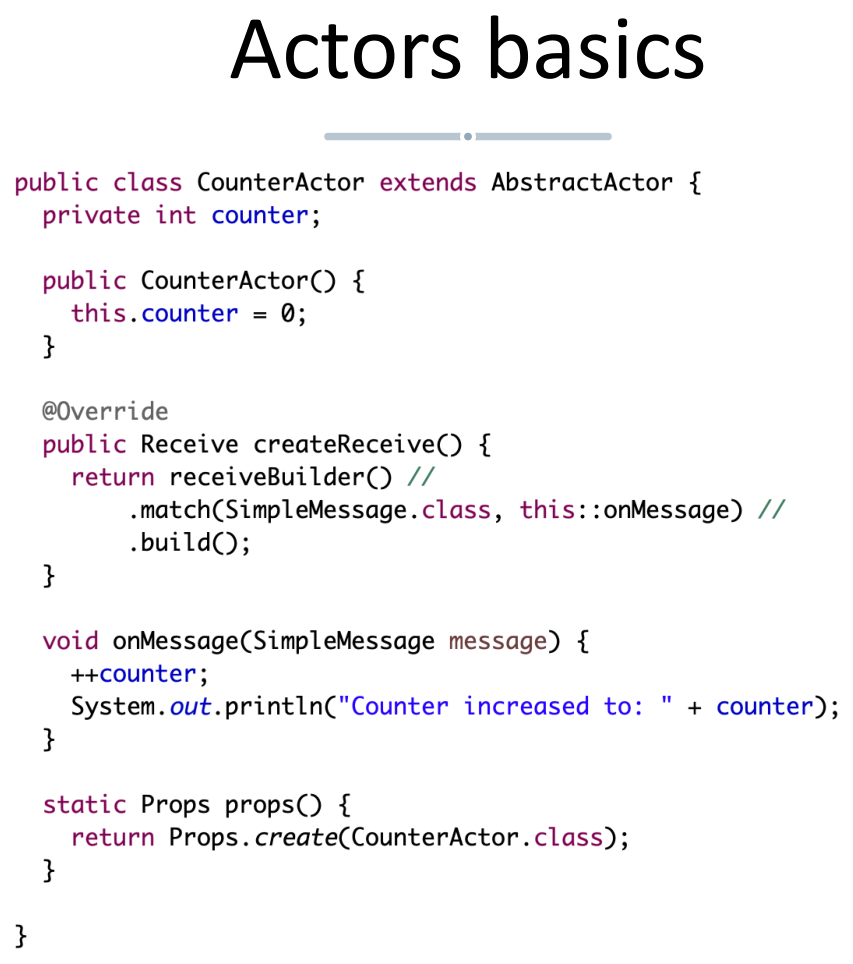
\includegraphics[width=0.65\textwidth]{img/chapter_01/deck1_slide_20.png}
\caption{Struttura architetturale di un Attore: i messaggi in arrivo si accodano nella Mailbox privata e vengono elaborati in sequenza senza interferenze concorrenti.}
\label{fig:actor_model_primitive_it}
\end{figure}

\subsection{Invarianti Fondamentali e Proprietà del Modello}
Le regole operative del modello ad attori garantiscono proprietà essenziali:
\begin{itemize}
    \item \textbf{Confinamento di Thread e Assenza di Stato Mutabile Condiviso}: Gli attori non condividono mai variabili. La comunicazione avviene esclusivamente tramite scambio asincrono di messaggi. Poiché ciascun attore elabora un singolo messaggio alla volta in modo sequenziale dalla propria mailbox, il corpo dell'attore è totalmente privo di corse critiche interne. Non occorre alcun blocco sincronizzato, mutex o primitiva atomica all'interno della logica di business.
    \item \textbf{Elaborazione Atomica del Messaggio}: Il ciclo di vita dell'elaborazione di un singolo messaggio è atomico rispetto allo stato dell'attore: il messaggio viene elaborato dall'inizio alla fine senza interleaving con altri messaggi indirizzati al medesimo attore. Eventuali messaggi ricevuti nel frattempo rimangono in coda nella mailbox.
    \item \textbf{Asincronismo Nativamente Non Bloccante}: La trasmissione dei messaggi è nativamente asincrona. Quando l'Attore $A$ invia un messaggio all'Attore $B$, $A$ non si blocca in attesa che $B$ lo riceva o lo elabori, ma prosegue immediatamente la propria esecuzione.
    \item \textbf{Stato e Persistenza}: Gli attori mantengono lo stato tra invocazioni successive. In estensioni persistenti (es. Akka Persistence), lo stato può essere salvato su supporti durevoli mediante tecniche di \textit{event sourcing} o snapshotting.
    \item \textbf{Trasparenza Spaziale e Topologica}: Gli attori interagiscono tramite riferimenti logici astratti (\textbf{ActorRef}), slegati dagli indirizzi di memoria fisici o dai descrittori di socket. La sintassi di comunicazione è identica sia che l'attore risieda sullo stesso core, nello stesso processo JVM, su una macchina differente della LAN o in un data center remoto.
\end{itemize}

\subsection{Adozione Industriale}
Il modello ad attori non costituisce una mera formulazione teorica, ma la spina dorsale di sistemi industriali ad altissima disponibilità e scalabilità:
\begin{itemize}
    \item \textbf{Erlang / OTP}: Sviluppato in Ericsson da Joe Armstrong per gestire centrali telefoniche con disponibilità richiesta del $99.9999999\%$ ("nove nove"). Costituisce l'infrastruttura di WhatsApp (miliardi di connessioni concorrenti con costi hardware minimi), Apache CouchDB e RabbitMQ.
    \item \textbf{Microsoft Orleans}: Framework a "virtual actors" alla base dei servizi cloud distribuiti per il multiplayer di videogiochi su scala globale come \textit{Halo}.
    \item \textbf{Akka (JVM - Java e Scala)}: Progettato da Jonas Bonér e Lightbend, fornisce un runtime per la Java Virtual Machine impiegato in sistemi di produzione mission-critical da aziende leader come BMW, Volkswagen Group, Siemens, Bosch e Volvo.
\end{itemize}

---

\section{L'Architettura di Akka su Piattaforma JVM}

\subsection{Componenti Fondamentali di Akka}
In ambiente JVM, Akka concretizza il modello ad attori mediante quattro astrazioni chiave:
\begin{enumerate}
    \item \textbf{ActorSystem}: Contenitore pesante e contesto radice dell'applicazione ad attori. Alloca e governa le risorse condivise, tra cui thread pool, dispatcher, parametri di configurazione, la mailbox dei Dead Letters e i servizi di scheduling. Tipicamente si istanzia un solo \texttt{ActorSystem} per processo JVM:
    \begin{lstlisting}[language=Java]
ActorSystem system = ActorSystem.create("NSDS-System");
    \end{lstlisting}
    \item \textbf{Props}: Oggetto immutabile di configurazione che incapsula la formula per la creazione di un attore, specificando la classe di appartenenza, i parametri del costruttore e il dispatcher designato.
    \item \textbf{ActorRef}: Riferimento logico immutabile e serializzabile all'attore. Il codice client e gli attori pari non interagiscono mai direttamente con l'oggetto Java concreto; ogni interazione è mediata dall'\texttt{ActorRef}. Un \texttt{ActorRef} rimane valido anche in caso di restart dell'attore a seguito di fallimento.
    \item \textbf{AbstractActor}: La classe base Java da estendere per definire la logica di ricezione dei messaggi mediante il metodo \texttt{createReceive()}.
\end{enumerate}

\begin{figure}[htbp]
\centering
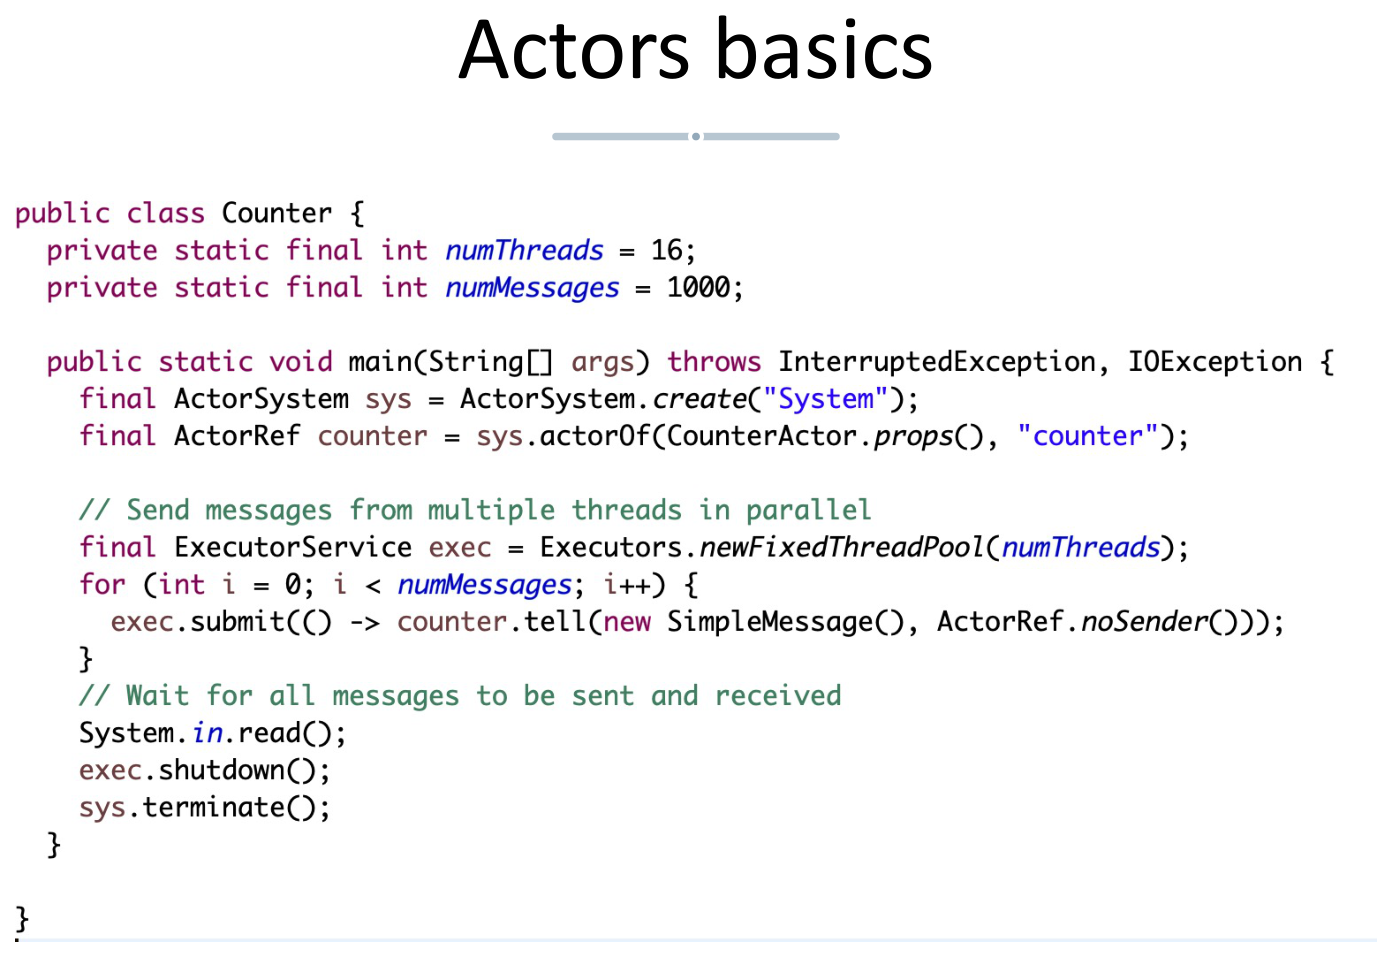
\includegraphics[width=0.75\textwidth]{img/chapter_01/deck1_slide_21.png}
\caption{Disaccoppiamento tra ActorRef, Mailbox e istanza dell'attore: l'interazione è sempre mediata dall'ActorRef a tutela dell'isolamento dello stato.}
\label{fig:actorref_decoupling_it}
\end{figure}

\subsection{Istanziazione degli Attori e Pattern Statico Props}
Per creare un attore, si invoca il metodo factory \texttt{actorOf} sull'\texttt{ActorSystem} (per attori top-level) o sul contesto locale \texttt{getContext()} (per attori figli), specificando un'istanza di \texttt{Props} e un identificatore univoco testuale.

È raccomandato definire un metodo factory statico \texttt{props()} all'interno della classe dell'attore:
\begin{lstlisting}[language=Java]
public class CounterActor extends AbstractActor {
    private int counter;

    public CounterActor(int initialValue) {
        this.counter = initialValue;
    }

    // Factory method statico per Props
    public static Props props(int initialValue) {
        return Props.create(CounterActor.class, () -> new CounterActor(initialValue));
    }

    @Override
    public Receive createReceive() {
        return receiveBuilder()
            .match(IncrementMessage.class, msg -> {
                this.counter += msg.getDelta();
            })
            .build();
    }
}
\end{lstlisting}

Nel codice principale:
\begin{lstlisting}[language=Java]
ActorSystem system = ActorSystem.create("ClusterSystem");
ActorRef counterRef = system.actorOf(CounterActor.props(0), "counterActor");
\end{lstlisting}

\subsection{Ciclo di Vita dell'Attore e Hook di Callback}
Un attore in Akka attraversa diverse fasi del ciclo di vita: \textbf{Starting}, \textbf{Receiving / Executing}, \textbf{Restarting} (in caso di guasto) e \textbf{Stopped}. Il framework mette a disposizione callback espliciti per la gestione delle risorse:

\begin{table}[htbp]
\centering
\small
\begin{tabularx}{\textwidth}{l p{4.5cm} X}
\toprule
\textbf{Metodo di Lifecycle} & \textbf{Momento di Invocazione} & \textbf{Semantica Operativa e Utilizzo Tipico} \\
\midrule
\texttt{preStart()} & Subito dopo la creazione dell'attore, prima di elaborare il primo messaggio. & Inizializzazione dello stato privato, apertura di socket o connessioni a database, pianificazione di messaggi periodici. \\
\midrule
\texttt{preRestart(reason, message)} & Invocato sull'istanza che ha fallito, prima della sua dismissione per riavvio. & Rilascio di risorse esterne; per default termina ricorsivamente tutti gli attori figli e invoca \texttt{postStop()}. \\
\midrule
\texttt{postRestart(reason)} & Invocato sulla nuova istanza subito dopo la ri-creazione a seguito di riavvio. & Re-inizializzazione dello stato per la nuova istanza; per default invoca \texttt{preStart()}. \\
\midrule
\texttt{postStop()} & Invocato dopo che l'attore è stato arrestato definitivamente. & Pulizia finale, rilascio di handle di sistema, notifica ai monitor remoti, salvataggio di buffer residui su disco. \\
\bottomrule
\end{tabularx}
\caption{Callback del Ciclo di Vita di un Attore Akka.}
\label{tab:lifecycle_hooks_it}
\end{table}

\begin{figure}[htbp]
\centering
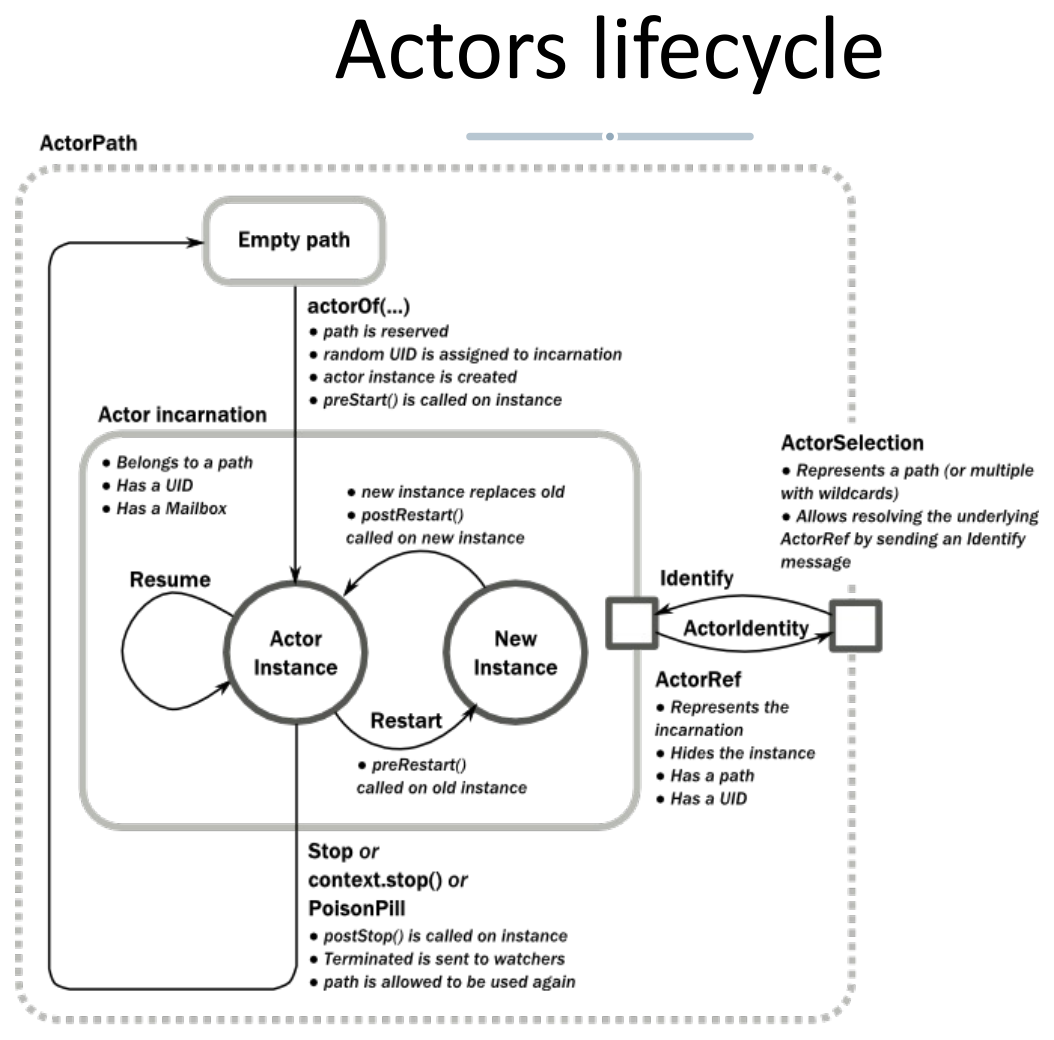
\includegraphics[width=0.7\textwidth]{img/chapter_01/actor_lifecycle.png}
\caption{Transizioni di stato del ciclo di vita di un attore in Akka, con evidenza del ciclo di riavvio controllato dal supervisore.}
\label{fig:actor_lifecycle_it}
\end{figure}

\subsection{Semantica della Mailbox e Requisito di Immutabilità}
Ogni attore possiede una propria \textbf{Mailbox}. L'implementazione di default è a capacità illimitata (\textit{unbounded}) e adotta una disciplina di accodamento \textbf{FIFO} per ciascuna coppia mittente-destinatario.

\subsubsection{Garanzie di Ordinamento}
In Akka, l'ordinamento soddisfa due garanzie formali:
\begin{enumerate}
    \item \textbf{Ordinamento FIFO tra Coppia Mittente-Destinatario}: Se l'Attore $A$ invia il messaggio $M_1$ e successivamente $M_2$ all'Attore $B$, $M_1$ sarà sempre recapitato ed elaborato da $B$ prima di $M_2$, a condizione che la trasmissione avvenga localmente o su connessione di rete affidabile punto-a-punto (come TCP):
    \begin{equation}
    \text{Invio}_A(M_1 \prec M_2) \implies \text{Ricezione}_B(M_1 \prec M_2)
    \end{equation}
    \item \textbf{Interleaving Non Deterministico da Mittenti Diversi}: Se l'Attore $A$ trasmette $M_A$ all'Attore $C$ e l'Attore $B$ trasmette $M_B$ all'Attore $C$, non esiste alcun vincolo di ordine relativo prefissato tra $M_A$ e $M_B$. L'ordine di accodamento dipenderà esclusivamente da latenze di rete e scheduling dei thread.
\end{enumerate}

\subsubsection{Il Vincolo di Immutabilità dei Messaggi}
Poiché gli attori residenti sulla medesima JVM condividono lo heap, i riferimenti agli oggetti messaggio vengono trasmessi come puntatori diretti per azzerare l'overhead di serializzazione. Ne deriva una regola categorica:
\begin{quote}
\textbf{Tutti i messaggi scambiati tra attori DEVONO essere rigorosamente immutabili.}
\end{quote}
Se un messaggio contenesse campi mutabili (es. setter pubblici, array o collezioni modificabili), thread differenti in esecuzione concorrente potrebbero leggere e mutare simultaneamente il carico utile, reintroducendo le medesime race condition e anomalie di memoria che il modello ad attori si prefigge di eliminare.

In Java, l'immutabilità va garantita a livello di codice con la seguente struttura:
\begin{lstlisting}[language=Java]
// Pattern canonico per un Messaggio Immutabile
public final class TemperatureReadingMsg implements Serializable {
    private final String sensorId;
    private final double temperature;
    private final long timestamp;

    public TemperatureReadingMsg(String sensorId, double temperature, long timestamp) {
        this.sensorId = sensorId;
        this.temperature = temperature;
        this.timestamp = timestamp;
    }

    public String getSensorId() { return sensorId; }
    public double getTemperature() { return temperature; }
    public long getTimestamp() { return timestamp; }
}
\end{lstlisting}

\subsubsection{Messaggi Non Gestiti e Dead Letters}
All'interno del blocco \texttt{createReceive()}, le clausole di matching vengono valutate nell'ordine sequenziale di dichiarazione. Qualora un messaggio in arrivo non soddisfi alcuna clausola definita, Akka invoca il gestore \texttt{unhandled(Object message)}, che per default inoltra il messaggio allo stream di eventi dei \textbf{Dead Letters} (\textit{Lettere Morte}). Anche i messaggi inviati ad attori arrestati confluiscono nei Dead Letters.

---

\section{Pattern di Comunicazione, Protocolli e Trasparenza di Posizione}

\subsection{Il Pattern Tell (Asincrono Fire-and-Forget)}
La primitiva fondamentale per la trasmissione di messaggi è \texttt{tell()}:
\begin{lstlisting}[language=Java]
targetActorRef.tell(message, senderActorRef);
\end{lstlisting}
L'operazione è asincrona e non bloccante: deposita il messaggio nella mailbox del destinatario e restituisce immediatamente il controllo al thread chiamante.

Regole operative:
\begin{itemize}
    \item \textbf{Identificazione del Mittente}: Se l'invio avviene dall'interno di un attore, specificare \texttt{self()} come secondo parametro consente al destinatario di replicare tramite \texttt{sender().tell(replyMsg, self())}.
    \item \textbf{Assenza di Mittente}: Se l'invio avviene dall'esterno del contesto attori (es. dal metodo \texttt{main}), si utilizza \texttt{ActorRef.noSender()}:
    \begin{lstlisting}[language=Java]
counterActor.tell(new IncrementMessage(1), ActorRef.noSender());
    \end{lstlisting}
    \item \textbf{Inoltro con Forwarding}: Un attore può inoltrare un messaggio a un terzo attore preservando l'indirizzo originale del mittente originario mediante \texttt{forward()}:
    \begin{lstlisting}[language=Java]
workerActor.forward(message, getContext());
    \end{lstlisting}
\end{itemize}

\subsection{Il Pattern Ask (Richiesta-Risposta con Future)}
Sebbene il \texttt{tell()} rappresenti il pattern puro, vi sono scenari in cui occorre interagire con confini applicativi non basati su attori (es. servire richieste HTTP sincrone, orchestrare test di integrazione o interrogare un attore dal \texttt{main}). In tali contesti si impiega il \textbf{Pattern Ask} via \texttt{akka.pattern.Patterns.ask}:

\begin{lstlisting}[language=Java]
import static akka.pattern.Patterns.ask;
import scala.concurrent.Future;
import scala.concurrent.Await;
import scala.concurrent.duration.Duration;
import java.util.concurrent.TimeUnit;

Duration timeout = Duration.create(3, TimeUnit.SECONDS);
Future<Object> future = ask(targetActorRef, new QueryBalanceMsg(accountId), 3000);

// Attesa bloccante (da limitare a test o confini esterni)
BalanceResponse reply = (BalanceResponse) Await.result(future, timeout);
\end{lstlisting}

\subsubsection{Meccanismo Interno e Costi Computazionali di Ask}
Internamente, il pattern Ask opera come segue:
\begin{enumerate}
    \item Akka alloca un \textbf{Promise Actor} temporaneo e usa-e-getta all'interno dell'\texttt{ActorSystem}.
    \item Il messaggio viene trasmesso al destinatario indicando il Promise Actor come \texttt{sender()}.
    \item Viene registrato un timer presso il servizio di scheduling per gestire il timeout prefissato.
    \item Quando il destinatario invoca \texttt{sender().tell(response, self())}, il Promise Actor intercetta la risposta, completa la \texttt{Future} e viene terminato.
    \item Se il timeout scade prima della risposta, la Future fallisce con \texttt{AskTimeoutException}.
\end{enumerate}

\begin{table}[htbp]
\centering
\small
\begin{tabularx}{\textwidth}{l X X}
\toprule
\textbf{Dimensione} & \textbf{Pattern Tell (\texttt{tell})} & \textbf{Pattern Ask (\texttt{ask})} \\
\midrule
\textbf{Modello di Esecuzione} & Totalmente asincrono, non bloccante (\textit{fire-and-forget}). & Asincrono basato su Future; bloccabile tramite \texttt{Await.result()}. \\
\midrule
\textbf{Overhead di Risorse} & Minimo: inserimento diretto nella mailbox del destinatario. & Medio: istanzia un Promise Actor temporaneo, un timer e un descrittore Future. \\
\midrule
\textbf{Gestione Guasti} & Trasparente: l'eventuale perdita o crash è gestita dal supervisore o via Dead Letters. & Esplicita: fallisce con \texttt{AskTimeoutException} in caso di timeout o mancata replica. \\
\midrule
\textbf{Ambito Elettivo} & Comunicazione ordinaria interna tra attori, pipeline ad alto throughput. & Interfacciamento con contesti esterni non ad attori (REST API, metodi di test \texttt{main}). \\
\bottomrule
\end{tabularx}
\caption{Analisi comparativa: Pattern Tell rispetto a Pattern Ask.}
\label{tab:tell_vs_ask_it}
\end{table}

\subsection{Garanzie di Consegna: Best-Effort (At-Most-Once)}
La teoria dei sistemi distribuiti dimostra che garantire la consegna esattamente una volta (\textit{exactly-once}) su reti inaffidabili senza coordinamento globale è impossibile (il paradosso dei due generali).

Akka adotta per impostazione predefinita una semantica \textbf{at-most-once (best-effort)}:
\begin{itemize}
    \item I messaggi possono andare perduti in caso di crash dell'attore, overflow della mailbox o partizione di rete.
    \item Il livello di trasporto non introduce duplicati arbitrari.
\end{itemize}

\textbf{Motivazione Architetturale ("Less is More")}:
Come spiegato dal Prof. Luca Mottola, imporre garanzie rigide di consegna a livello di trasporto richiede un costo sproporzionato: sequenziamento dei pacchetti, acknowledgment, buffer di ritrasmissione, persistenza su disco e tabelle di deduplicazione. In ambiente distribuito:
\begin{enumerate}
    \item Il protocollo IP è nativamente best-effort.
    \item TCP fornisce flussi affidabili su singola connessione, ma non può mascherare crash di sistema, partizioni o riavvii dei processi.
    \item Molti domini operativi gestiscono dati temporalmente deperibili o idempotenti (es. letture di sensori, dove un dato perso è reso obsoleto dal valore successivo).
    \item I requisiti che esigono garanzie superiori possono essere soddisfatti implementando acknowledgment a livello applicativo o integrando code persistenti dedicate (come Apache Kafka).
\end{enumerate}

\subsection{Trasparenza di Posizione e Akka Remoting}
La \textbf{Trasparenza di Posizione} (\textit{Location Transparency}) costituisce uno dei massimi punti di forza di Akka: un \texttt{ActorRef} astrae la locazione fisica dell'attore. Il programmatore invia messaggi con la medesima sintassi \texttt{ref.tell(msg, self())} a prescindere dal fatto che il destinatario si trovi sulla JVM locale o su un server remoto.

\subsubsection{Actor Path e Indirizzamento Gerarchico}
Ogni attore è identificato univocamente da un URI gerarchico strutturato come segue:
\begin{equation}
\texttt{akka.<protocollo>://<nome-actor-system>@<hostname>:<porta>/user/<percorso-gerarchico>}
\end{equation}
Esempi:
\begin{itemize}
    \item Percorso locale: \texttt{akka://NSDS-System/user/supervisor/worker-1}
    \item Percorso remoto su TCP: \texttt{akka.tcp://ClusterNode@192.168.1.100:2552/user/dataProcessor}
\end{itemize}

\subsubsection{Configurazione Remota via HOCON}
I parametri di networking si configurano tramite file HOCON (\texttt{application.conf}):
\begin{lstlisting}
akka {
  actor {
    provider = remote
  }
  remote {
    enabled-transports = ["akka.remote.netty.tcp"]
    netty.tcp {
      hostname = "127.0.0.1"
      port = 6123
    }
  }
}
\end{lstlisting}

\subsubsection{Risoluzione di Attori Remoti: ActorSelection}
Per contattare un attore remoto di cui non si possiede preventivamente l'\texttt{ActorRef}, si interroga l'URI logico tramite \texttt{actorSelection()}:
\begin{lstlisting}[language=Java]
// Ricerca del server remoto da parte del client
String remoteAddress = "akka.tcp://ServerSystem@127.0.0.1:6123/user/serverActor";
ActorSelection remoteSelection = getContext().actorSelection(remoteAddress);

// Invio diretto alla selezione logica
remoteSelection.tell(new QueryMessage("data"), getSelf());
\end{lstlisting}
Al momento della risposta, il mittente remoto recapita il proprio \texttt{ActorRef} concreto all'interno del campo \texttt{sender()}, abilitando le successive comunicazioni dirette ad alte prestazioni.

---

\section{Modifica Dinamica del Comportamento e Meccanismo di Stash}

\subsection{Macchine a Stati Finiti con Become e Unbecome}
In molti protocolli distribuiti, un attore deve modificare radicalmente la propria logica di gestione dei messaggi in funzione dello stato operativo in cui si trova (es. transizione tra gli stati \textit{Disconnesso}, \textit{In Connessione}, \textit{Attivo}, \textit{Occupato} o \textit{Sospeso}).

Anziché ricorrere a catene condizionali complesse e fragili (\texttt{if-else} o \texttt{switch} su flag di stato interni), Akka consente all'attore di sostituire l'intero blocco di ricezione a runtime mediante \texttt{getContext().become()}:

\begin{lstlisting}[language=Java]
public class ProtocolActor extends AbstractActor {

    @Override
    public Receive createReceive() {
        return disconnectedBehavior();
    }

    private Receive disconnectedBehavior() {
        return receiveBuilder()
            .match(ConnectMsg.class, msg -> {
                System.out.println("Connessione a " + msg.getHost());
                getContext().become(connectedBehavior());
            })
            .match(DataMsg.class, msg -> {
                System.err.println("Dati rifiutati: attore non connesso!");
            })
            .build();
    }

    private Receive connectedBehavior() {
        return receiveBuilder()
            .match(DataMsg.class, msg -> {
                System.out.println("Dati elaborati: " + msg.getPayload());
            })
            .match(DisconnectMsg.class, msg -> {
                System.out.println("Disconnessione in corso...");
                getContext().become(disconnectedBehavior());
            })
            .build();
    }
}
\end{lstlisting}

Se si passa il valore booleano \texttt{false} come secondo argomento a \texttt{become(newReceive, false)}, Akka non scarta il vecchio comportamento, ma lo inserisce in uno stack interno. Invocando successivamente \texttt{getContext().unbecome()}, l'attore ripristina istantaneamente il comportamento precedente.

\subsection{Il Buffer di Stash: AbstractActorWithStash}
Capita frequentemente che un attore, in un dato stato, riceva messaggi che non può gestire immediatamente, ma che non devono essere persi. Il pattern di \textbf{Stash} consente all'attore di accantonare temporaneamente tali messaggi in un buffer secondario per poi rielaborarli al momento opportuno.

Per implementare lo stash, l'attore deve:
\begin{enumerate}
    \item Estendere la classe \texttt{AbstractActorWithStash}.
    \item Invocare il metodo \texttt{stash()} sui messaggi da differire: il messaggio corrente viene rimosso dal ciclo di elaborazione e appeso in coda allo stash.
    \item Quando l'attore commuta in uno stato abilitato a processarli, invocare il metodo \texttt{unstashAll()}.
\end{enumerate}

\subsubsection{Riposizionamento dei Messaggi nella Mailbox}
All'invocazione di \texttt{unstashAll()}, Akka preleva tutti i messaggi accumulati nello stash e li reinserisce nella mailbox:
\begin{quote}
\textbf{I messaggi estratti dallo Stash vengono reinseriti in TESTA alla Mailbox primaria, preservando l'ordine relativo con cui sono stati accantonati.}
\end{quote}
Questo meccanismo assicura che i messaggi differiti vengano elaborati con priorità rispetto a nuovi messaggi sopraggiunti nel frattempo.

\begin{figure}[htbp]
\centering
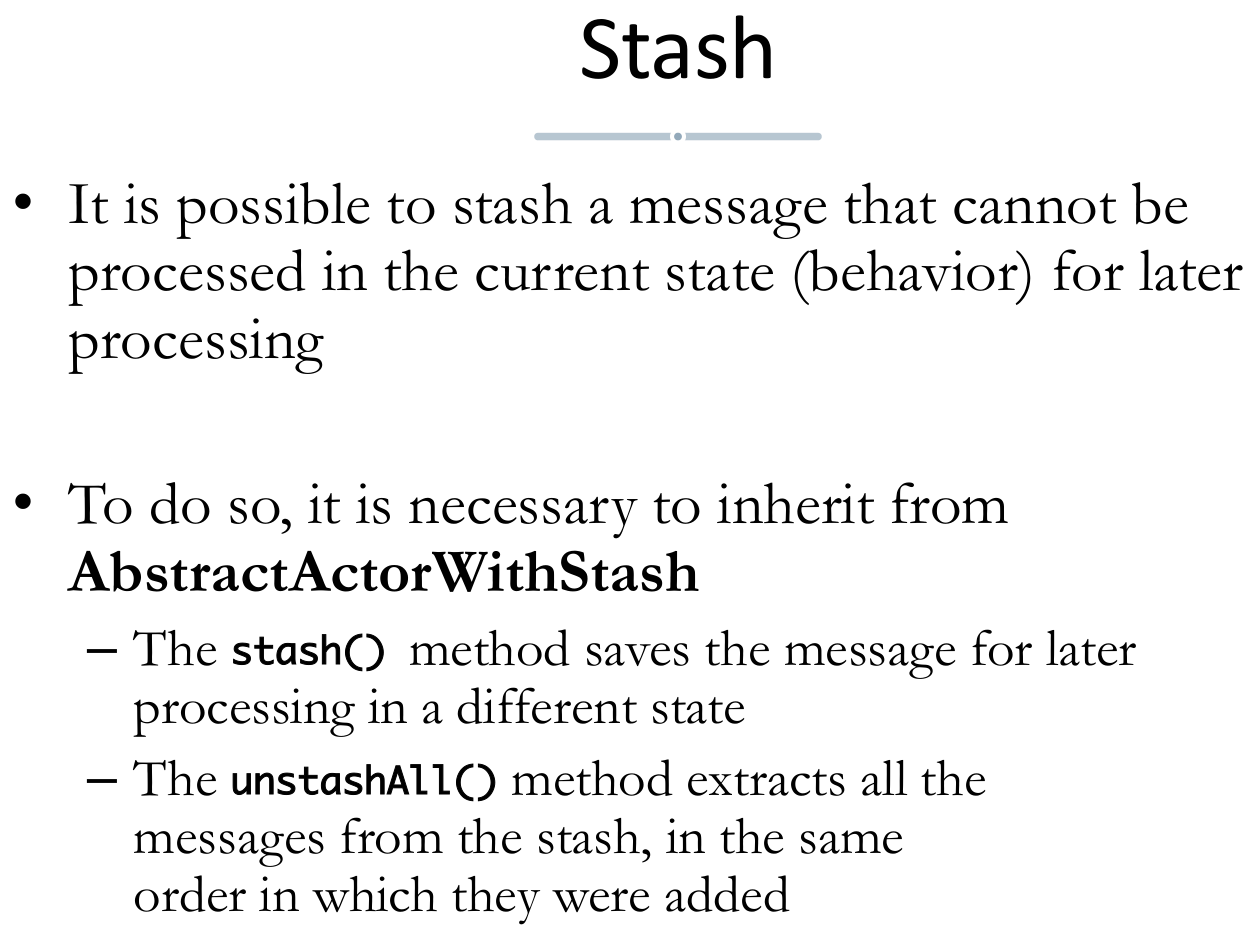
\includegraphics[width=0.75\textwidth]{img/chapter_01/stash_mechanics.png}
\caption{Funzionamento dello Stash: accantonamento temporaneo e reinserimento prioritario in testa alla Mailbox principale al momento del cambio di stato.}
\label{fig:stash_mechanics_it}
\end{figure}

---

\section{Tolleranza ai Guasti e Gerarchia di Supervisione}

\subsection{La Filosofia "Let It Crash"}
Nei linguaggi orientati agli oggetti tradizionali (come Java standard), la gestione delle eccezioni è intrecciata alla logica funzionale mediante blocchi difensivi \texttt{try-catch}. Se un'eccezione non prevista sale lungo lo stack di chiamate, il thread muore in modo incontrollato, rischiando di lasciare strutture dati corrotte o lock bloccati per sempre.

Il modello ad attori sposa la filosofia di Joe Armstrong nota come \textbf{"Let It Crash"} (\textit{lascia che si guasti}):
\begin{itemize}
    \item \textbf{Separazione tra Logica di Business e Gestione Errori}: Lo sviluppatore non implementa codice difensivo per intercettare anomalie fatali all'interno dell'elaborazione funzionale. Se si verifica un'eccezione non recuperabile localmente, l'attore lancia l'errore e si arresta.
    \item \textbf{Supervisione Esterna}: La gestione del guasto è interamente esternalizzata. Il genitore gerarchico dell'attore—il suo \textbf{Supervisore}—viene notificato automaticamente dal runtime e applica una direttiva strategica di ripristino.
\end{itemize}

\subsection{La Struttura Gerarchica degli Attori}
In Akka, nessun attore vive isolato: essi sono organizzati in un albero gerarchico rigoroso. Ogni attore creato tramite \texttt{getContext().actorOf()} è figlio dell'attore che lo ha generato.

\begin{figure}[htbp]
\centering
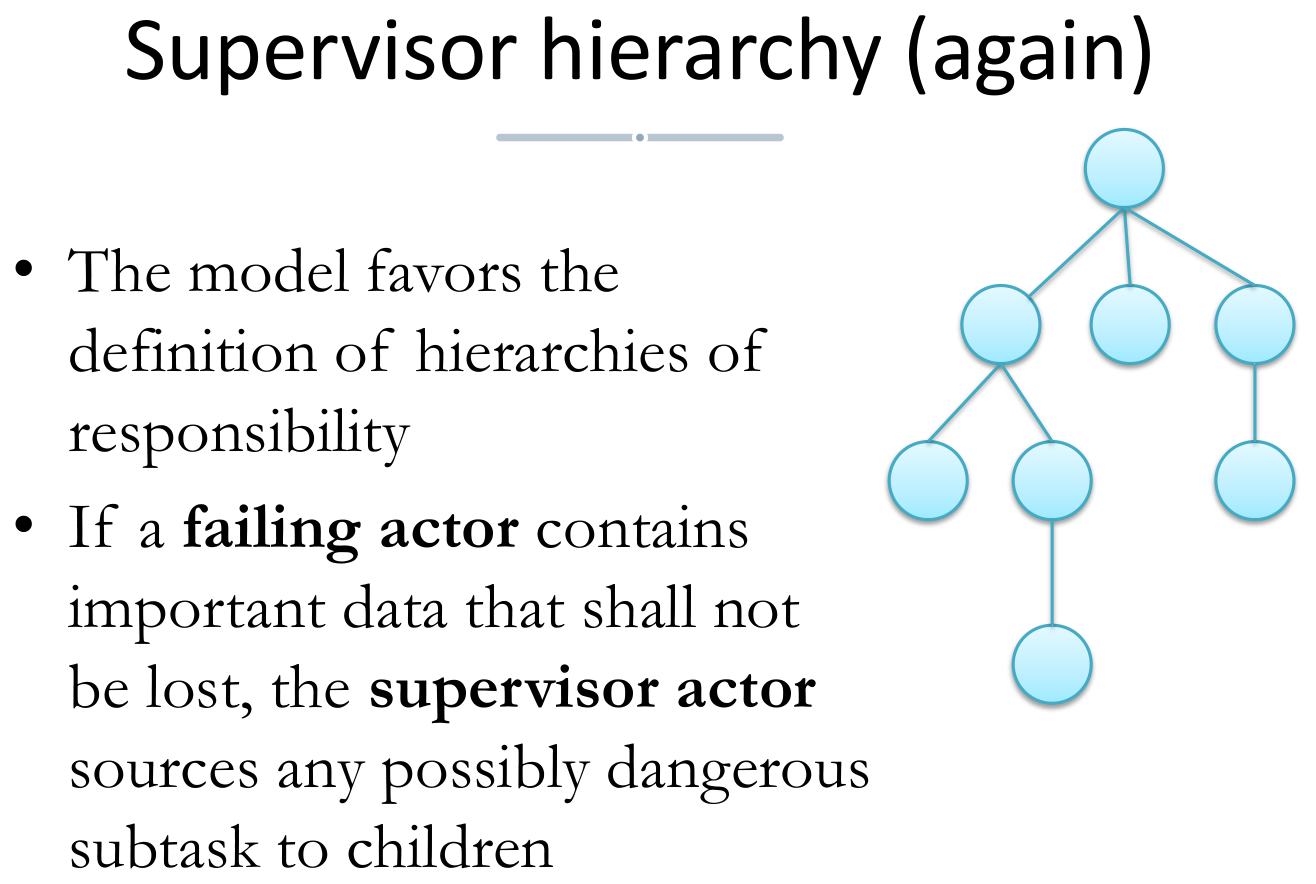
\includegraphics[width=0.75\textwidth]{img/chapter_01/deck3_slide_6.png}
\caption{Albero di Supervisione in Akka: suddivisione tra guardiano di sistema, guardiano utente (/user) e gerarchia applicativa.}
\label{fig:supervision_hierarchy_it}
\end{figure}

La gerarchia poggia su tre vertici principali:
\begin{enumerate}
    \item \textbf{Root Guardian (\texttt{/})}: Vertice supremo dell'intero runtime.
    \item \textbf{System Guardian (\texttt{/system})}: Sovrintende ai servizi infrastrutturali di framework (logging, socket di remoting, dead letters).
    \item \textbf{User Guardian (\texttt{/user})}: Genitore diretto di tutti gli attori applicativi creati via \texttt{system.actorOf()}.
\end{enumerate}

\subsection{Strategie di Supervisione e Direttive di Recupero}
Un attore supervisore stabilisce la propria politica di resilienza sovrascrivendo il metodo \texttt{supervisorStrategy()}, restituendo un'istanza di \texttt{OneForOneStrategy} o di \texttt{AllForOneStrategy}:

\begin{itemize}
    \item \textbf{OneForOneStrategy}: La direttiva di recupero scelta dal supervisore viene applicata \textbf{esclusivamente} all'attore figlio che ha sollevato l'errore. Gli altri attori figli continuano la loro normale attività senza interruzione. È la strategia d'elezione per carichi di lavoro indipendenti.
    \item \textbf{AllForOneStrategy}: La direttiva di recupero viene applicata a \textbf{tutti} gli attori figli del supervisore, anche se uno solo di essi ha manifestato il guasto. Questa strategia è indispensabile qualora i figli collaborino a una transazione coordinata in cui il guasto di un membro rende nullo o incoerente lo stato dei compagni.
\end{itemize}

\subsubsection{Le Quattro Direttive di Supervisione}
All'intercettazione del fallimento di un figlio, il supervisore applica una tra quattro direttive canoniche:
\begin{enumerate}
    \item \textbf{Resume}: L'attore guasto \textbf{non} viene terminato. Il suo stato interno in memoria viene integralmente conservato e l'attore procede immediatamente all'elaborazione del messaggio successivo presente nella mailbox.
    \begin{itemize}
        \item \textit{Caso d'uso}: Errori transitori o non correlati a corruzione di stato (es. un pacchetto con formato non valido da scartare, un temporaneo timeout di rete).
    \end{itemize}
    \item \textbf{Restart} (\textit{Politica di Default}): L'istanza dell'attore che ha fallito viene distrutta e una nuova istanza viene generata a partire dai \texttt{Props} originali.
    \begin{itemize}
        \item \textit{Semantica di Stato}: Lo stato privato viene integralmente ripristinato ai valori iniziali del costruttore.
        \item \textit{Semantica di Mailbox}: La mailbox viene \textbf{preservata}. I messaggi pendenti rimangono in coda e verranno elaborati dalla nuova istanza appena creata.
        \item \textit{Hook Invocati}: Sulla vecchia istanza si esegue \texttt{preRestart(reason, message)}; sulla nuova istanza si esegue \texttt{postRestart(reason)}.
        \item \textit{Caso d'uso}: Corruzione di stato interno o eccezioni inattese non gestibili localmente.
    \end{itemize}
    \item \textbf{Stop}: L'attore viene arrestato definitivamente. La mailbox viene svuotata (i messaggi residui finiscono nei Dead Letters), i suoi eventuali figli vengono ricorsivamente terminati e il relativo \texttt{ActorRef} cessa di essere utilizzabile.
    \begin{itemize}
        \item \textit{Caso d'uso}: Esaurimento fatale di risorse o errori irreversibili di configurazione.
    \end{itemize}
    \item \textbf{Escalate}: Il supervisore riconosce di non avere la competenza logica per gestire quel tipo di eccezione; sospende se stesso e tutti i suoi figli e ri-lancia l'errore al proprio genitore lungo la gerarchia.
\end{enumerate}

\subsubsection{Implementazione della Strategia in Java}
Il codice seguente illustra la configurazione di una \texttt{OneForOneStrategy} con limiti sul numero massimo di tentativi di riavvio in una finestra temporale mobile:

\begin{lstlisting}[language=Java]
import akka.actor.AbstractActor;
import akka.actor.OneForOneStrategy;
import akka.actor.SupervisorStrategy;
import akka.japi.pf.DeciderBuilder;
import java.time.Duration;

public class CustomSupervisorActor extends AbstractActor {

    // Massimo 10 riavvii consentiti nell'arco di 1 minuto
    private static final SupervisorStrategy STRATEGY = new OneForOneStrategy(
        10,
        Duration.ofMinutes(1),
        DeciderBuilder
            .match(IllegalArgumentException.class, e -> SupervisorStrategy.resume())
            .match(NullPointerException.class, e -> SupervisorStrategy.restart())
            .match(IllegalStateException.class, e -> SupervisorStrategy.stop())
            .matchAny(e -> SupervisorStrategy.escalate())
            .build()
    );

    @Override
    public SupervisorStrategy supervisorStrategy() {
        return STRATEGY;
    }

    @Override
    public Receive createReceive() {
        return receiveBuilder()
            .match(Props.class, childProps -> {
                ActorRef child = getContext().actorOf(childProps);
                sender().tell(child, self());
            })
            .build();
    }
}
\end{lstlisting}

---

\section{Akka Clustering e Topologie Distribuite}

\subsection{Architettura Decentralizzata di Cluster Membership}
Akka Cluster estende la trasparenza di posizione su un insieme dinamico di macchine di rete senza fare affidamento su coordinatori centralizzati (quali Apache ZooKeeper):
\begin{itemize}
    \item \textbf{Topologia Peer-to-Peer Simmetrica}: Tutti i nodi partecipano su base paritaria; non esiste alcun singolo punto di fallimento (\textit{Single Point of Failure - SPOF}) né collo di bottiglia centrale.
    \item \textbf{Protocollo Gossip}: Lo stato di appartenenza al cluster è propagato in modo asincrono tramite scambi casuali di stato tra coppie di nodi.
    \item \textbf{Failure Detection Distribuito}: Monitoraggio automatico e continuo della raggiungibilità dei nodi.
\end{itemize}

\subsection{Il Protocollo Gossip e la Convergenza con Vector Clock}
I nodi formano una rete di overlay. A cadenza periodica (default: 1 secondo), ciascun nodo seleziona a caso un altro membro del cluster e scambia la propria vista di appartenenza.
\begin{itemize}
    \item \textbf{Vector Clock per la Causalità}: Ogni messaggio di gossip include un \textbf{Vector Clock} che traccia l'ordine causale parziale delle mutazioni di stato (nodi che entrano, escono o divengono non raggiungibili).
    \item \textbf{Convergenza del Gossip}: Un nodo raggiunge la convergenza quando può verificare matematicamente che tutti i membri raggiungibili del cluster condividono la medesima vista di appartenenza.
    \item \textbf{Il Ruolo del Leader}: Le transizioni di topologia (es. la promozione di un nodo da \textit{Joining} a \textit{Up}) possono essere decise unicamente dal \textbf{Cluster Leader} eletto, una volta che sia stata accertata la piena convergenza del gossip su tutti i nodi raggiungibili.
\end{itemize}

\subsection{Ciclo di Vita del Nodo e Failure Detector $\Phi$-Accrual}
Uno stato di nodo nel cluster evolve formalmente secondo la sequenza:
\begin{equation}
\text{Joining} \longrightarrow \text{Up} \longrightarrow \text{Leaving} \longrightarrow \text{Exiting} \longrightarrow \text{Down} \longrightarrow \text{Removed}
\end{equation}

\subsubsection{Il $\Phi$ Accrual Failure Detector}
Akka adotta il \textbf{$\Phi$ Accrual Failure Detector} (sviluppato da Hayashibara et al.). Anziché operare decisioni binarie (attivo/spento) basate su timeout rigidi di heartbeat, il detector raccoglie una cronologia statistica degli intervalli di inter-arrivo dei battiti cardiaci, adattandoli a una distribuzione normale. Restituisce una variabile continua di sospetto $\Phi$:
\begin{equation}
\Phi = -\log_{10}(P_{\text{later}}(t - t_{\text{last}}))
\end{equation}
In caso di momentanea congestione di rete, $\Phi$ sale gradualmente. Se $\Phi$ supera una soglia configurata (default: 10), il nodo viene contrassegnato come \textbf{Unreachable} (Non Raggiungibile). La presenza di nodi non raggiungibili blocca la convergenza finché il nodo non ripristina la connettività o viene marcato come \textbf{Down}.

\subsection{Seed Node e Strumenti di Alto Livello}
\begin{itemize}
    \item \textbf{Seed Nodes}: Indirizzi di contatto preconfigurati usati come punti di rendezvous per i nuovi nodi che intendono entrare nel cluster.
    \item \textbf{Cluster Singleton}: Assicura che esista una sola istanza al mondo di un determinato attore all'interno dell'intero cluster, con failover trasparente in caso di crash del nodo ospitante.
    \item \textbf{Cluster Sharding}: Partiziona automaticamente un vasto insieme di attori con stato sui vari nodi del cluster, instradando i messaggi alla destinazione corretta sulla base dell'identificatore di entità.
    \item \textbf{Distributed Data}: Replica lo stato tra nodi impiegando tipi di dati privi di conflitti (\textit{Conflict-Free Replicated Data Types - CRDT}), consentendo modifiche concorrenti prive di lock che convergono deterministicamente.
\end{itemize}

---

\section{Analisi Critica, Complessità e Trade-off Architetturali}

\subsection{Analisi Quantitativa delle Risorse e Complessità}

\begin{table}[htbp]
\centering
\small
\begin{tabularx}{\textwidth}{l p{3.5cm} X}
\toprule
\textbf{Metrica / Dimensione} & \textbf{Limite Quantitativo} & \textbf{Analisi Architetturale e Trade-off} \\
\midrule
\textbf{Occupazione di Memoria} & $\approx 300 - 500$ byte per istanza di Attore. & A fronte di un thread di sistema operativo ($\approx 1$ MB di stack), è possibile allocare milioni di attori all'interno dello heap standard della JVM. \\
\midrule
\textbf{Complessità di Trasmissione} & $O(1)$ punto-a-punto; \newline $O(N)$ multicast. & Il recapito locale equivale al passaggio diretto di un puntatore; il recapito remoto richiede una singola scrittura su socket TCP. \\
\midrule
\textbf{Latenza di Convergenza Gossip} & $O(\log N)$ round in un cluster di $N$ nodi. & La propagazione dell'informazione scala logaritmicamente con il numero di nodi; l'overhead di heartbeat è strettamente limitato. \\
\midrule
\textbf{Colli di Bottiglia Concorrenti} & Zero contese di lock nell'attore. & L'unico collo di bottiglia insorge se la frequenza di arrivo dei messaggi supera stabilmente la velocità sequenziale di elaborazione dell'attore. \\
\midrule
\textbf{Costo di Ripristino da Guasto} & Restart: riallocazione $O(1)$. & Il riavvio preserva la mailbox già accodata, minimizzando la perdita di messaggi durante il ripristino da guasti transitori. \\
\bottomrule
\end{tabularx}
\caption{Caratteristiche Prestazionali e Consumo Risorse in Akka.}
\label{tab:system_complexity_it}
\end{table}

\subsection{Trade-off Architetturali Fondamentali}
Nella progettazione di sistemi distribuiti su Akka, gli ingegneri affrontano scelte architetturali critiche:
\begin{enumerate}
    \item \textbf{Dimensionamento dei Dispatcher e Operazioni Bloccanti}: Gli attori condividono thread pool sottostanti (ForkJoin o ThreadPoolExecutor). Qualora un attore esegua un'operazione bloccante (es. query JDBC sincrona, chiamate I/O bloccanti), i thread del pool vengono saturati, impedendo l'esecuzione di attori del tutto indipendenti. \textit{Soluzione}: Isolare le chiamate bloccanti su un thread pool dedicato tramite Future.
    \item \textbf{Dimensionamento della Mailbox (Unbounded vs Bounded)}: Una mailbox a capacità illimitata assorbe picchi temporanei senza scartare pacchetti, ma espone al rischio di \texttt{OutOfMemoryError} in caso di saturazione cronica. Mailbox limitate (\textit{bounded}) tutelano la memoria ma richiedono strategie esplicite di scarto (\textit{drop}) o contropressione.
    \item \textbf{Granularità della Supervisione}: Gerarchie profonde isolano precisamente il raggio di impatto dei guasti (\textit{blast radius}), ma comportano una modesta latenza di attraversamento dell'albero gerarchico.
\end{enumerate}

---

\section{Domande di Ripasso ed Esercizi d'Esame Risolti (Politecnico di Milano)}

\subsection{Domande Teoriche di Verifica}

\paragraph{Domanda 1: Quali sono le differenze operative tra le direttive di supervisione Resume e Restart? In quale scenario applicativo un ingegnere deve tassativamente optare per la Resume?}
\textbf{Soluzione:}
All'atto dell'intercettazione di un'eccezione, se il supervisore applica la direttiva \texttt{Resume}, l'istanza dell'attore in memoria \textbf{non viene distrutta}. Il suo stato interno e tutte le sue variabili private rimangono intatti, e l'attore passa immediatamente a elaborare il messaggio successivo in coda nella mailbox.

Al contrario, con la direttiva \texttt{Restart}:
\begin{enumerate}
    \item L'istanza dell'attore che ha sollevato l'errore viene de-allocata (invocando l'hook \texttt{preRestart(reason, message)}).
    \item Viene istanziato un nuovo oggetto attore a partire dai \texttt{Props} iniziali, invocando \texttt{postRestart(reason)}.
    \item Lo stato interno dell'attore viene azzerato e re-inizializzato ai valori di default del costruttore.
    \item La mailbox viene preservata intatta e la nuova istanza prosegue elaborando i messaggi pendenti.
\end{enumerate}
\textit{Criterio di Scelta}: L'ingegnere deve impiegare tassativamente la direttiva \texttt{Resume} quando il fallimento è causato da un dato malformato o da un'anomalia esterna transitoria che non ha corrotto le strutture dati interne dell'attore (es. una lettura di temperatura non valida o un messaggio sconosciuto). In tale contesto, lo stato storico accumulato (es. la media progressiva delle misure corrette o la mappa delle sottoscrizioni dei client) è prezioso e non deve essere resettato.

\paragraph{Domanda 2: Per quale ragione i messaggi in Akka devono essere rigorosamente immutabili e in cosa differiscono i meccanismi interni del pattern Ask rispetto al pattern Tell?}
\textbf{Soluzione:}
All'interno della medesima JVM, Akka ottimizza la comunicazione passando direttamente i riferimenti agli oggetti messaggio tra le mailbox per evitare il gravoso overhead di serializzazione. Se i messaggi fossero mutabili, più thread che servono attori distinti potrebbero accedere e modificare contemporaneamente gli stessi campi di memoria, scatenando race condition, problemi di visibilità di cache e incoerenze di stato.

L'operazione \texttt{tell()} è un'interazione asincrona \textit{fire-and-forget}: si limita ad accodare il messaggio nella mailbox del destinatario e ritorna istantaneamente. Il pattern \texttt{ask()} crea invece un \textit{Promise Actor} effimero di sistema, avvia un timer per il timeout prefissato, imposta tale attore fittizio come mittente e restituisce una \texttt{Future}. L'Ask comporta un maggiore consumo di risorse di memoria e scheduling e rischia di degradare le prestazioni se atteso in modo bloccante con \texttt{Await.result()}.

---

\subsection{Soluzione Evaluation Lab 2022: Broker Pub/Sub con Partizionamento e Batching Dinamico}

\subsubsection{Specifica del Problema}
Progettare un sistema Publish-Subscribe distribuito in Akka costituito da:
\begin{itemize}
    \item \textbf{Due Worker Actor}: Verificano la corrispondenza tra eventi pubblicati e sottoscrizioni registrate.
    \item \textbf{Un Broker Actor}: Supervisiona e coordina i worker, partizionando le registrazioni sulla base della parità della chiave (chiavi pari assegnate al Worker 1, chiavi dispari al Worker 2).
    \item \textbf{Tolleranza ai Guasti}: Quando un worker riceve un messaggio \texttt{PublishMsg} per un topic mai registrato in precedenza, solleva un'eccezione. Il broker deve supervisionare i worker applicando una strategia che preservi l'insieme delle sottoscrizioni attive prima del guasto (\texttt{Resume}).
    \item \textbf{Batching Dinamico}: Alla ricezione di un messaggio \texttt{BatchMsg(isOn = true)}, il broker deve commutare comportamento e accumulare i messaggi di evento in arrivo. Alla ricezione di \texttt{BatchMsg(isOn = false)}, tutti gli eventi accumulati nel buffer devono essere inoltrati ed elaborati in blocco.
\end{itemize}

\begin{figure}[htbp]
\centering
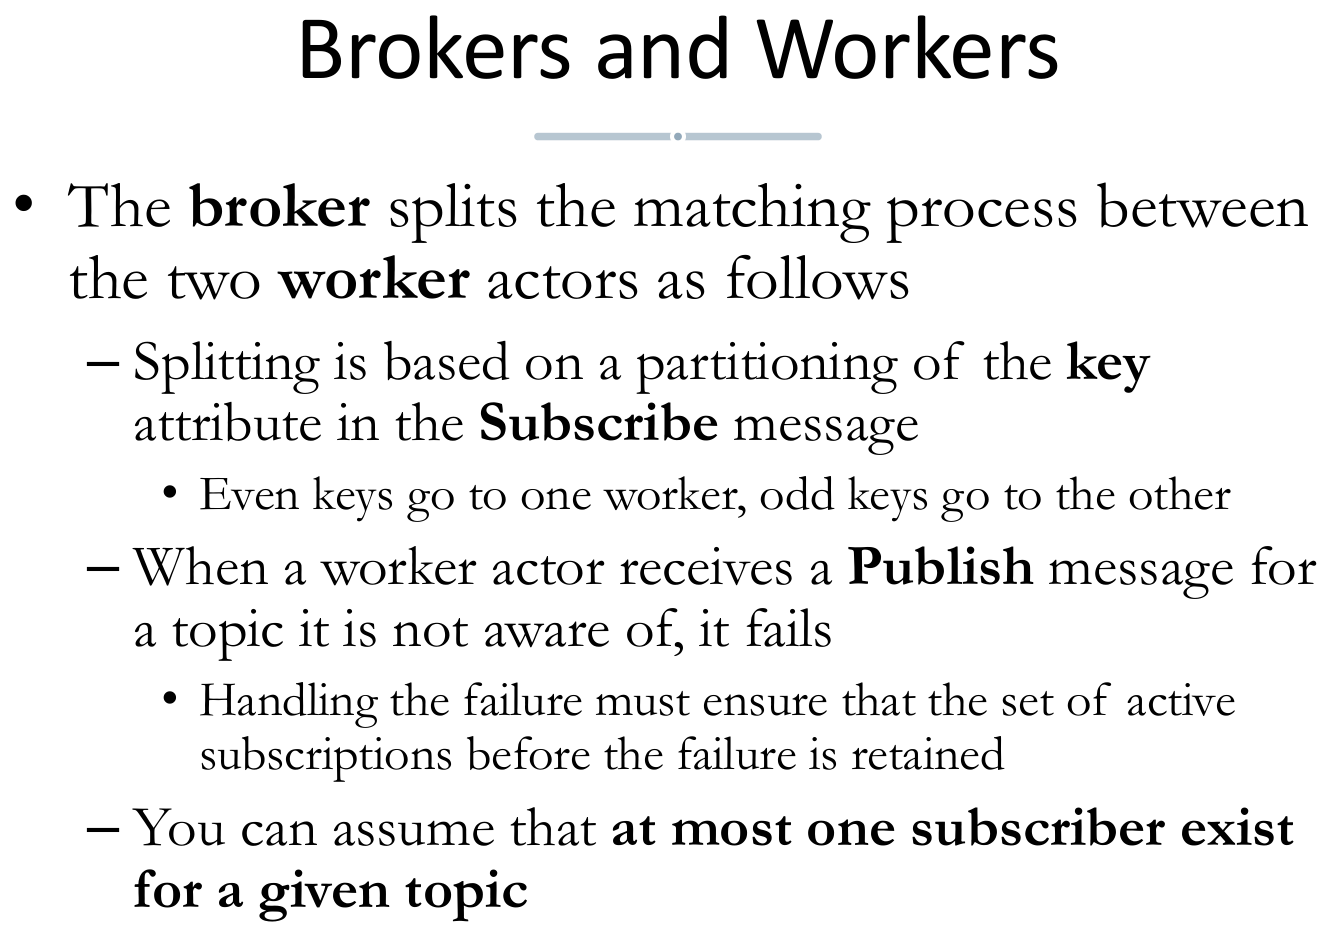
\includegraphics[width=0.75\textwidth]{img/chapter_01/eval22_pubsub_architecture.png}
\caption{Architettura dell'Evaluation Lab 2022: Broker con partizionamento su worker pari/dispari, accumulo batch e supervisione Resume.}
\label{fig:eval22_architecture_it}
\end{figure}

\subsubsection{Implementazione Completa in Codice Java}

\begin{lstlisting}[language=Java, caption={Definizione dei Messaggi del Sistema Pub/Sub}]
import akka.actor.ActorRef;
import java.io.Serializable;

public class Messages {
    public static class SubscribeMsg implements Serializable {
        private final String topic;
        private final int key;
        private final ActorRef subscriber;

        public SubscribeMsg(String topic, int key, ActorRef subscriber) {
            this.topic = topic;
            this.key = key;
            this.subscriber = subscriber;
        }
        public String getTopic() { return topic; }
        public int getKey() { return key; }
        public ActorRef getSubscriber() { return subscriber; }
    }

    public static class PublishMsg implements Serializable {
        private final String topic;
        private final int key;
        private final String payload;

        public PublishMsg(String topic, int key, String payload) {
            this.topic = topic;
            this.key = key;
            this.payload = payload;
        }
        public String getTopic() { return topic; }
        public int getKey() { return key; }
        public String getPayload() { return payload; }
    }

    public static class NotifyMsg implements Serializable {
        private final String payload;
        public NotifyMsg(String payload) { this.payload = payload; }
        public String getPayload() { return payload; }
    }

    public static class BatchMsg implements Serializable {
        private final boolean on;
        public BatchMsg(boolean on) { this.on = on; }
        public boolean isOn() { return on; }
    }
}
\end{lstlisting}

\begin{lstlisting}[language=Java, caption={WorkerActor con Gestione Guasti su Topic Non Registrati}]
import akka.actor.AbstractActor;
import akka.actor.Props;
import java.util.HashMap;
import java.util.Map;

public class WorkerActor extends AbstractActor {
    // Mappa delle sottoscrizioni: Topic -> Riferimento Sottoscrittore
    private final Map<String, ActorRef> subscriptions = new HashMap<>();

    public static Props props() {
        return Props.create(WorkerActor.class, WorkerActor::new);
    }

    @Override
    public Receive createReceive() {
        return receiveBuilder()
            .match(Messages.SubscribeMsg.class, msg -> {
                subscriptions.put(msg.getTopic(), msg.getSubscriber());
                System.out.println(self().path().name() + " ha registrato il topic: " + msg.getTopic());
            })
            .match(Messages.PublishMsg.class, msg -> {
                if (!subscriptions.containsKey(msg.getTopic())) {
                    System.err.println(self().path().name() + " fallimento: topic sconosciuto " + msg.getTopic());
                    throw new Exception("Topic sconosciuto: " + msg.getTopic());
                }
                ActorRef sub = subscriptions.get(msg.getTopic());
                sub.tell(new Messages.NotifyMsg(msg.getPayload()), self());
            })
            .build();
    }
}
\end{lstlisting}

\begin{lstlisting}[language=Java, caption={BrokerActor con Switch Dinamico del Comportamento e Supervisione Resume}]
import akka.actor.*;
import akka.japi.pf.DeciderBuilder;
import java.time.Duration;
import java.util.LinkedList;
import java.util.Queue;

public class BrokerActor extends AbstractActorWithStash {
    private final ActorRef workerEven;
    private final ActorRef workerOdd;
    private final Queue<Messages.PublishMsg> batchBuffer = new LinkedList<>();

    // Politica di supervisione: Resume per preservare le registrazioni attive
    private static final SupervisorStrategy STRATEGY = new OneForOneStrategy(
        10,
        Duration.ofMinutes(1),
        DeciderBuilder
            .match(Exception.class, e -> SupervisorStrategy.resume())
            .build()
    );

    @Override
    public SupervisorStrategy supervisorStrategy() {
        return STRATEGY;
    }

    public BrokerActor() {
        this.workerEven = getContext().actorOf(WorkerActor.props(), "workerEven");
        this.workerOdd = getContext().actorOf(WorkerActor.props(), "workerOdd");
    }

    public static Props props() {
        return Props.create(BrokerActor.class, BrokerActor::new);
    }

    @Override
    public Receive createReceive() {
        return normalBehavior();
    }

    // Comportamento Ordinario: instradamento immediato
    private Receive normalBehavior() {
        return receiveBuilder()
            .match(Messages.BatchMsg.class, msg -> {
                if (msg.isOn()) {
                    System.out.println("Broker: passaggio alla modalita BATCH.");
                    getContext().become(batchBehavior());
                }
            })
            .match(Messages.SubscribeMsg.class, this::routeSubscription)
            .match(Messages.PublishMsg.class, this::routePublish)
            .build();
    }

    // Comportamento Batch: accumulo degli eventi nel buffer
    private Receive batchBehavior() {
        return receiveBuilder()
            .match(Messages.BatchMsg.class, msg -> {
                if (!msg.isOn()) {
                    System.out.println("Broker: rilascio batch (" + batchBuffer.size() + " messaggi).");
                    while (!batchBuffer.isEmpty()) {
                        routePublish(batchBuffer.poll());
                    }
                    getContext().become(normalBehavior());
                }
            })
            .match(Messages.SubscribeMsg.class, this::routeSubscription)
            .match(Messages.PublishMsg.class, batchBuffer::add)
            .build();
    }

    private void routeSubscription(Messages.SubscribeMsg msg) {
        if (msg.getKey() % 2 == 0) {
            workerEven.forward(msg, getContext());
        } else {
            workerOdd.forward(msg, getContext());
        }
    }

    private void routePublish(Messages.PublishMsg msg) {
        if (msg.getKey() % 2 == 0) {
            workerEven.forward(msg, getContext());
        } else {
            workerOdd.forward(msg, getContext());
        }
    }
}
\end{lstlisting}

---

\subsection{Soluzione Evaluation Lab 2023: Monitoraggio Sensori con Criteri di Smistamento}

\subsubsection{Specifica del Problema}
Sviluppare un'architettura in Akka per il monitoraggio di sensori industriali composta da:
\begin{enumerate}
    \item \textbf{Attori SensorDataProcessor}: Mantengono la media progressiva delle letture di temperatura ricevute:
    \begin{equation}
    \bar{T}_{k} = \frac{(k-1)\bar{T}_{k-1} + T_k}{k}
    \end{equation}
    Se un processore riceve un valore di temperatura negativo ($T < 0$), solleva un'eccezione. La gestione del guasto deve garantire che la media calcolata fino a quel momento venga preservata e che la lettura errata venga scartata dal computo (\texttt{Resume}).
    \item \textbf{Un Attore DispatcherActor}: Instrada dinamicamente le letture in arrivo secondo due strategie selezionabili via messaggio \texttt{DispatchLogicMsg}:
    \begin{itemize}
        \item \textbf{Load Balancing}: Associa stabilmente ciascun sensore al processore che gestisce il minor numero di sensori, garantendo bilanciamento del carico.
        \item \textbf{Round Robin}: Distribuisce a rotazione circolare ogni nuova lettura ricevuta tra i processori disponibili.
    \end{itemize}
\end{enumerate}

\begin{figure}[htbp]
\centering
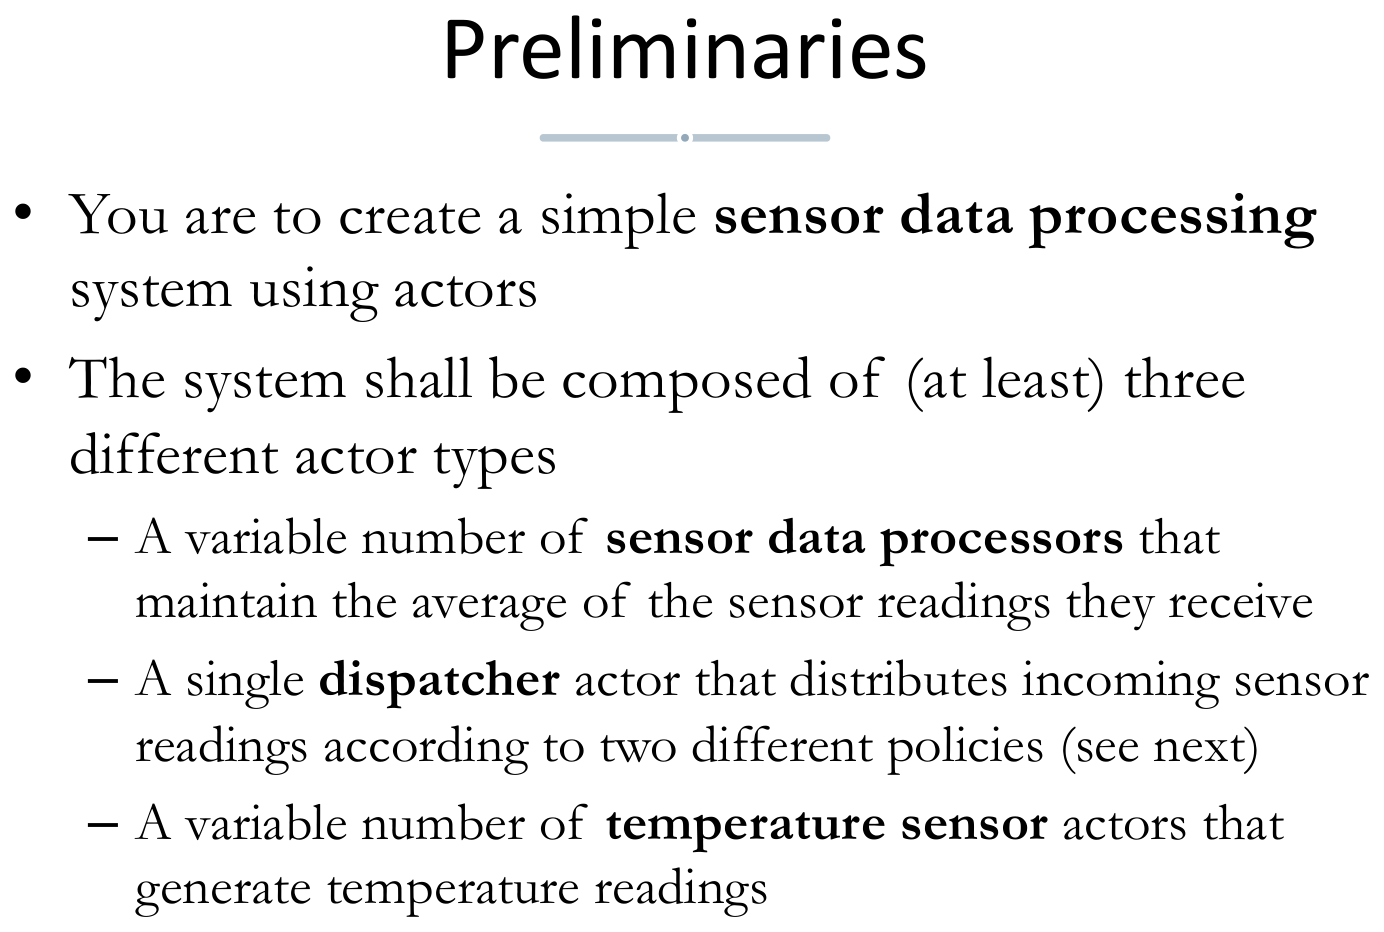
\includegraphics[width=0.75\textwidth]{img/chapter_01/eval23_sensor_architecture.png}
\caption{Architettura dell'Evaluation Lab 2023: Dispatcher con switch di smistamento Round Robin / Load Balancing e processori resilienti con Resume.}
\label{fig:eval23_architecture_it}
\end{figure}

\subsubsection{Implementazione Completa in Codice Java}

\begin{lstlisting}[language=Java, caption={SensorProcessorActor con Preservazione della Media Storica}]
import akka.actor.AbstractActor;
import akka.actor.Props;

public class SensorProcessorActor extends AbstractActor {
    private double sum = 0.0;
    private int count = 0;

    public static Props props() {
        return Props.create(SensorProcessorActor.class, SensorProcessorActor::new);
    }

    @Override
    public Receive createReceive() {
        return receiveBuilder()
            .match(TemperatureMsg.class, msg -> {
                if (msg.getValue() < 0) {
                    System.err.println(self().path().name() + " rifiuta temperatura non valida: " + msg.getValue());
                    throw new IllegalArgumentException("Temperatura negativa non ammessa: " + msg.getValue());
                }
                count++;
                sum += msg.getValue();
                double currentAvg = sum / count;
                System.out.printf("%s -> Misura: %.2f | Nuova Media: %.2f (Campioni totali: %d)%n",
                    self().path().name(), msg.getValue(), currentAvg, count);
            })
            .build();
    }
}
\end{lstlisting}

\begin{lstlisting}[language=Java, caption={DispatcherActor con Politiche di Routing e Strategia di Supervisione}]
import akka.actor.*;
import akka.japi.pf.DeciderBuilder;
import java.time.Duration;
import java.util.*;

public class DispatcherActor extends AbstractActor {
    private final List<ActorRef> processors;
    private final Map<ActorRef, ActorRef> sensorToProcessorMap = new HashMap<>();
    private final Map<ActorRef, Integer> processorLoadMap = new HashMap<>();
    private int roundRobinIndex = 0;
    private boolean isRoundRobin = true; // Politica di default

    private static final SupervisorStrategy STRATEGY = new OneForOneStrategy(
        10,
        Duration.ofMinutes(1),
        DeciderBuilder
            .match(IllegalArgumentException.class, e -> SupervisorStrategy.resume())
            .build()
    );

    @Override
    public SupervisorStrategy supervisorStrategy() {
        return STRATEGY;
    }

    public DispatcherActor(int numProcessors) {
        this.processors = new ArrayList<>();
        for (int i = 0; i < numProcessors; i++) {
            ActorRef p = getContext().actorOf(SensorProcessorActor.props(), "processor-" + i);
            processors.add(p);
            processorLoadMap.put(p, 0);
        }
    }

    public static Props props(int numProcessors) {
        return Props.create(DispatcherActor.class, () -> new DispatcherActor(numProcessors));
    }

    @Override
    public Receive createReceive() {
        return receiveBuilder()
            .match(DispatchLogicMsg.class, msg -> {
                this.isRoundRobin = msg.isRoundRobin();
                System.out.println("Dispatcher: logica commutata in " + 
                    (isRoundRobin ? "ROUND ROBIN" : "LOAD BALANCING"));
            })
            .match(TemperatureMsg.class, msg -> {
                ActorRef targetProcessor;
                if (isRoundRobin) {
                    targetProcessor = processors.get(roundRobinIndex);
                    roundRobinIndex = (roundRobinIndex + 1) % processors.size();
                } else {
                    ActorRef sensorSender = sender();
                    if (!sensorToProcessorMap.containsKey(sensorSender)) {
                        // Individua il processore con il carico minore di sensori
                        targetProcessor = processors.stream()
                            .min(Comparator.comparingInt(processorLoadMap::get))
                            .orElse(processors.get(0));
                        sensorToProcessorMap.put(sensorSender, targetProcessor);
                        processorLoadMap.put(targetProcessor, processorLoadMap.get(targetProcessor) + 1);
                    } else {
                        targetProcessor = sensorToProcessorMap.get(sensorSender);
                    }
                }
                targetProcessor.forward(msg, getContext());
            })
            .build();
    }
}
\end{lstlisting}

